%%%%%%%%%%%%%%%%%%%%%%%%%%%%%%%%%%%%%%%%%%%%%%%%
% Corrigé UPSTI
% Concours - Epreuve - Année
%%%%%%%%%%%%%%%%%%%%%%%%%%%%%%%%%%%%%%%%%%%%%%%%
\documentclass[11pt]{article}

%%%%%%%%%%%%%%%%%%%%%%%%%%%%%%%%%%%%%%%%%%%%%%%%
% Package UPSTI_Document
%%%%%%%%%%%%%%%%%%%%%%%%%%%%%%%%%%%%%%%%%%%%%%%% 
\usepackage{UPSTI_Corrige_Concours}	% Squelette minimal
%\usepackage[UPSTI]{UPSTI_Corrige_Concours} % Chargement des packages UPSTI  (téléchargeables ici: https://www.upsti.fr/documents-pedagogiques/upsti-kit-de-demarrage-latex)

%---------------------------------%
% Packages personnalisés
%---------------------------------%
% Insérez ici les packages que vous utilisez habituellement

%%%%%%%%%%%%
% Définition des vecteurs 
%%%%%%%%%%%%
\newcommand{\vect}[1]{\overrightarrow{#1}}
\newcommand{\axe}[2]{\left(#1,\vect{#2}\right)}
\newcommand{\couple}[2]{\left(#1,\vect{#2}\right)}
\newcommand{\angl}[2]{\left(\vect{#1},\vect{#2}\right)}

\newcommand{\rep}[1]{\mathcal{R}_{#1}}
\newcommand{\quadruplet}[4]{\left(#1;#2,#3,#4 \right)}
\newcommand{\repere}[4]{\left(#1;\vect{#2},\vect{#3},\vect{#4} \right)}
\newcommand{\base}[3]{\left(\vect{#1},\vect{#2},\vect{#3} \right)}


\newcommand{\vx}[1]{\vect{x_{#1}}}
\newcommand{\vy}[1]{\vect{y_{#1}}}
\newcommand{\vz}[1]{\vect{z_{#1}}}

% d droit pour le calcul différentiel
\newcommand{\dd}{\text{d}}

\newcommand{\inertie}[2]{I\left({#1}, #2\right)}
\newcommand{\matinertie}[7]{
\begin{pmatrix}
#1 & #6 & #5 \\
#6 & #2 & #4 \\
#5 & #4 & #3 \\
\end{pmatrix}_{#7}}
%%%%%%%%%%%%
% Définition des torseurs 
%%%%%%%%%%%%

\newcommand{\ec}[2]{%
\mathcal{E}_{c\;#1/#2}}

\newcommand{\pext}[3]{%
\mathcal{P}_{#1\rightarrow#2/#3}}

\newcommand{\pint}[3]{%
\mathcal{P}_{#1 \stackrel{\text{#3}}{\leftrightarrow} #2 }}


 \newcommand{\torseur}[1]{%
\left\{{#1}\right\}
}

\newcommand{\torseurcin}[3]{%
\left\{\mathcal{#1} \left(#2/#3 \right) \right\}
}

\newcommand{\torseurci}[2]{%
\left\{\sigma \left(#1/#2 \right) \right\}
}
\newcommand{\torseurdyn}[2]{%
\left\{\mathcal{D} \left(#1/#2 \right) \right\}
}


\newcommand{\torseurstat}[3]{%
\left\{\mathcal{#1} \left(#2\rightarrow #3 \right) \right\}
}


 \newcommand{\torseurc}[8]{%
%\left\{#1 \right\}=
\left\{
{#1}
\right\}
 = 
\left\{%
\begin{array}{cc}%
{#2} & {#5}\\%
{#3} & {#6}\\%
{#4} & {#7}\\%
\end{array}%
\right\}_{#8}%
}

 \newcommand{\torseurcol}[7]{
\left\{%
\begin{array}{cc}%
{#1} & {#4}\\%
{#2} & {#5}\\%
{#3} & {#6}\\%
\end{array}%
\right\}_{#7}%
}

 \newcommand{\torseurl}[3]{%
%\left\{\mathcal{#1}\right\}_{#2}=%
\left\{%
\begin{array}{l}%
{#1} \\%
{#2} %
\end{array}%
\right\}_{#3}%
}

% Vecteur vitesse
 \newcommand{\vectv}[3]{%
\vect{V_{{#2}/{#3}}}\left( {#1}\right)
}

% Vecteur force
\newcommand{\vectf}[2]{%
\vect{R_{ {#1} \rightarrow {#2}}}
}

% Vecteur moment stat
\newcommand{\vectm}[3]{%
\vect{\mathcal{M}_{{#2} \rightarrow {#3}}}    \left( {#1}\right)
}




% Vecteur résultante cin
\newcommand{\vectrc}[2]{%
\vect{R_{c\;{{#1}/ {#2}}}}
}
% Vecteur moment cin
\newcommand{\vectmc}[3]{%
\vect{\sigma_{{#2}/{#3}}}\left( {#1}\right)
}


% Vecteur résultante dyn
\newcommand{\vectrd}[2]{%
\vect{R_{d\;{{#1}/ {#2}}}}
}
% Vecteur moment dyn
\newcommand{\vectmd}[3]{%
\vect{\delta_{{#2}/{#3}}}\left( {#1}\right)
}

% Vecteur accélération
 \newcommand{\vectg}[3]{%
\vect{\Gamma_{{#2}/{#3}}}\left( {#1}\right)
}

% Vecteur omega
 \newcommand{\vecto}[2]{%
\vect{\Omega_{{#1}/{#2}}}
}
% }$$\left\{\mathcal{#1} \right\}_{#2} =%
% \left\{%
% \begin{array}{c}%
%  #3 \\%
%  #4 %
% \end{array}%
% \right\}_{#5}}


%% 
% Boite pour Python
\usepackage{listingsutf8}
\lstset{
	language={Python},
	columns=flexible,
	basicstyle=\ttfamily,
	keywordstyle=\color{blue}, % je voudrais mettre les mots-clé en gras (\bfseries) mais c'est incompatible avec typewriter
	commentstyle=\color{gray}, % commentaires
	%backgroundcolor=\color{green!10}, % couleur du fond
	backgroundcolor=\color{white}, % couleur du fond
	%frame=single, rulecolor=\color{green!10}, % encadrement + couleur de l'encadrement
	frame=single, rulecolor=\color{white}, % encadrement + couleur de l'encadrement
	%numbers=left, numberstyle=\tiny, stepnumber=1, numbersep=5pt,
	showstringspaces=false, % supprime les espaces apparents dans les lignes de texte
	stringstyle=\color{red!50}\itshape,
	inputencoding=utf8,
	extendedchars=true,
   literate=
  {á}{{\'a}}1 {é}{{\'e}}1 {í}{{\'i}}1 {ó}{{\'o}}1 {ú}{{\'u}}1
  {Á}{{\'A}}1 {É}{{\'E}}1 {Í}{{\'I}}1 {Ó}{{\'O}}1 {Ú}{{\'U}}1
  {à}{{\`a}}1 {è}{{\`e}}1 {ì}{{\`i}}1 {ò}{{\`o}}1 {ù}{{\`u}}1
  {À}{{\`A}}1 {È}{{\'E}}1 {Ì}{{\`I}}1 {Ò}{{\`O}}1 {Ù}{{\`U}}1
  {ä}{{\"a}}1 {ë}{{\"e}}1 {ï}{{\"i}}1 {ö}{{\"o}}1 {ü}{{\"u}}1
  {Ä}{{\"A}}1 {Ë}{{\"E}}1 {Ï}{{\"I}}1 {Ö}{{\"O}}1 {Ü}{{\"U}}1
  {â}{{\^a}}1 {ê}{{\^e}}1 {î}{{\^i}}1 {ô}{{\^o}}1 {û}{{\^u}}1
  {Â}{{\^A}}1 {Ê}{{\^E}}1 {Î}{{\^I}}1 {Ô}{{\^O}}1 {Û}{{\^U}}1
  {œ}{{\oe}}1 {Œ}{{\OE}}1 {æ}{{\ae}}1 {Æ}{{\AE}}1 {ß}{{\ss}}1
  {ű}{{\H{u}}}1 {Ű}{{\H{U}}}1 {ő}{{\H{o}}}1 {Ő}{{\H{O}}}1
  {ç}{{\c c}}1 {Ç}{{\c C}}1 {ø}{{\o}}1 {å}{{\r a}}1 {Å}{{\r A}}1
  {€}{{\EUR}}1 {£}{{\pounds}}1
}
\usepackage{amsmath}

\usepackage{siunitx}
\sisetup{output-decimal-marker = {,}}

% Boite pour Python
\usepackage{listingsutf8}
\lstset{
	language={Python},
	columns=flexible,
	basicstyle=\ttfamily,
	keywordstyle=\color{blue}, % je voudrais mettre les mots-clé en gras (\bfseries) mais c'est incompatible avec typewriter
	commentstyle=\color{gray}, % commentaires
	%backgroundcolor=\color{green!10}, % couleur du fond
	backgroundcolor=\color{white}, % couleur du fond
	%frame=single, rulecolor=\color{green!10}, % encadrement + couleur de l'encadrement
	frame=single, rulecolor=\color{white}, % encadrement + couleur de l'encadrement
	%numbers=left, numberstyle=\tiny, stepnumber=1, numbersep=5pt,
	showstringspaces=false, % supprime les espaces apparents dans les lignes de texte
	stringstyle=\color{red!50}\itshape,
	inputencoding=utf8,
	extendedchars=true,
   literate=
  {á}{{\'a}}1 {é}{{\'e}}1 {í}{{\'i}}1 {ó}{{\'o}}1 {ú}{{\'u}}1
  {Á}{{\'A}}1 {É}{{\'E}}1 {Í}{{\'I}}1 {Ó}{{\'O}}1 {Ú}{{\'U}}1
  {à}{{\`a}}1 {è}{{\`e}}1 {ì}{{\`i}}1 {ò}{{\`o}}1 {ù}{{\`u}}1
  {À}{{\`A}}1 {È}{{\'E}}1 {Ì}{{\`I}}1 {Ò}{{\`O}}1 {Ù}{{\`U}}1
  {ä}{{\"a}}1 {ë}{{\"e}}1 {ï}{{\"i}}1 {ö}{{\"o}}1 {ü}{{\"u}}1
  {Ä}{{\"A}}1 {Ë}{{\"E}}1 {Ï}{{\"I}}1 {Ö}{{\"O}}1 {Ü}{{\"U}}1
  {â}{{\^a}}1 {ê}{{\^e}}1 {î}{{\^i}}1 {ô}{{\^o}}1 {û}{{\^u}}1
  {Â}{{\^A}}1 {Ê}{{\^E}}1 {Î}{{\^I}}1 {Ô}{{\^O}}1 {Û}{{\^U}}1
  {œ}{{\oe}}1 {Œ}{{\OE}}1 {æ}{{\ae}}1 {Æ}{{\AE}}1 {ß}{{\ss}}1
  {ű}{{\H{u}}}1 {Ű}{{\H{U}}}1 {ő}{{\H{o}}}1 {Ő}{{\H{O}}}1
  {ç}{{\c c}}1 {Ç}{{\c C}}1 {ø}{{\o}}1 {å}{{\r a}}1 {Å}{{\r A}}1
  {€}{{\EUR}}1 {£}{{\pounds}}1
}

% ---

%---------------------------------%
% Paramètres du corrigé
%---------------------------------%

% ----------
% Concours
% ----------
% 0: Custom*
% 1: ATS
% 2: Banque PT
% 3: CCINP
% 4: CCP
% 5: CCS (par défaut)
% 6: E3A
% 7: ICNA
% 8: Mines AADN
% 9: Mines Ponts
% 10: X-ENS
% * Si on met la valeur 0, il faut décommenter la ligne suivante: 		
%\newcommand{\UPSTIconcoursCustom}{Concours custom}
\newcommand{\UPSTIidConcours}{5}

% ----------
% Filière
% ----------
% 0: Custom*
% 1: ATS
% 2: MP
% 3: MPI
% 4: PSI (par défaut)
% 5: PT
% 6: TSI
% 7: MP2I
% 8: MPSI
% 9: PCSI
% 10: PTSI
% * Si on met la valeur 0, il faut décommenter la ligne suivante: 		
%\newcommand{\UPSTIfiliereCustom}{Filière custom}
\newcommand{\UPSTIidFiliere}{4}

% ----------
% Epreuve
% ----------
% 0: Custom*
% 1: S2I (par défaut)
% 2: Informatique
% 3: Modélisation et informatique
% 4: Modélisation
% 5: Physique - SI
% 6: SI A
% 7: SI B
% 8: SI C
% 9: SI 1
% 10: SI 2
% * Si on met la valeur 0, il faut décommenter la ligne suivante: 		
%\newcommand{\UPSTIepreuveCustom}{Epreuve custom}
\newcommand{\UPSTIidEpreuve}{1}

% ----------
% Session
% ----------
\newcommand{\UPSTIsession}{2020}

% ----------
% Titre de l'épreuve (souvent, le nom du support)
% ----------
\newcommand{\UPSTItitreEpreuve}{Robotisation du désherbage mécanique des vignes}
% Si le nom est trop long pour l'entête, on peu décommenter la ligne suivante:
\newcommand{\UPSTItitreEpreuveRaccourci}{Robot Bakus}      

%----------------------------------------------- 
\UPSTIprepareDocument		% "Compile" les variables
%%%%%%%%%%%%%%%%%%%%%%%%%%%%%%%%%%%%%%%%%%%%%%%% 


%%%%%%%%%%%%%%%%%%%%%%%%%%%%%%%%%%%%%%%%%%%%%%%% 
% Début du document
%%%%%%%%%%%%%%%%%%%%%%%%%%%%%%%%%%%%%%%%%%%%%%%% 
\begin{document}
\UPSTIpreambuleEpreuve	% Affichage du préambule de l'épreuve

%---------------------------------%
% DEBUT du contenu
%---------------------------------%

%\UPSTItitrePartieCorrige{Titre de la partie}


\UPSTIquestion À partir des équations (E3), (I.1), (I.2) et (I.3) établies à partir du modèle cinématique étendu de la
figure A, montrer que : 
$$ \begin{array}{lr}
y'_F = \theta + \delta_F-\beta_F   & \text{(I.4)} \\
y'_R = \theta + \delta_R-\beta_R  & \text{(I.5)}\\
\theta'=\dfrac{y'_F-y'_R}{2L}       & \text{(I.6)}
\end{array}.$$

\begin{UPSTIcorrige}


On a les résultats suivants :  $  \theta = \dfrac{ y_{R} - y_F}{2L }$ (E3), d'après  (I.1), (I.2) et (I.3), $\dot{x}_{G_2}=V_{G_2}$, $\dot{y_F}=V_{G_2}\left(\theta + \delta_F - \beta_F\right)$ et  $\dot{y_R}=V_{G_2}\left(\theta + \delta_R - \beta_R\right)$. 


D'après (I.1), $\dot{x}_{G_2}= \dfrac{\dd x_{G_2}}{\dd t} =  V_{G_2}$.
Par ailleurs (\textbf{à confirmer}) on cherche $y'_F=\dfrac{\dd y_F}{\dd x_{G_2}} $ 
$= \dfrac{\dd y_F}{\dd t}  \cdot \dfrac{\dd  t}{\dd x_{G_2}}$ 
$ =\dot{y_F}\cdot \dfrac{1}{V_{G_2}}$ 
$ =\theta + \delta_F - \beta_F$.

On montre de même que $y'_R = \theta + \delta_R-\beta_R$

Enfin, $\theta' = \dfrac{\dd \theta}{\dd x_{G_2}}=\dfrac{ \dfrac{\dd y_{R}}{\dd x_{G_2}} - \dfrac{\dd y_F}{\dd x_{G_2}}}{2L } = \dfrac{y'_R-y'_F}{2L}$.

\textbf{Attention : le sujet propose l'opposé de ce résultat.}

\end{UPSTIcorrige}

\subsubsection{Asservissement de la variable de déplacement latéral $y_F$ à une consigne $y^*_F=0$}

\UPSTIobjectif{Justifier le choix du modèle du comportement en déplacement latéral $y_F$ du robot assurant sa convergence à une valeur de consigne $y_F^*$ et son réglage}

\UPSTIquestion Par analogie avec un modèle temporel usuel d’ordre 2 à identifier, de paramètres caractéristiques $\omega_{0F}$, $\xi_F$ et $K_F$ :
\begin{itemize}
\item en justifiant la réponse, tracer l’allure de l’évolution de  $y_F\left(x_{G_2}\right)$  imposée par le modèle 1 (I.7) pour une consigne $y_F^*=0$ en fonction de $x_{G_2}$, lorsque $y_F\left(x_{G_2}=0\right)=y_{F0}>0$
 ($y_{F0}$ étant une valeur constante), $y'_F\left(x_{G_2}=0\right)=0$, $K_{pF}=\dfrac{K^2_{dF}}{4}$ et $K_{dF}\simeq 5$; 
 \item préciser sur le graphe les éléments caractéristiques de la courbe tracée pour $x_{G_2}=0$ ;
\item justifier pourquoi le paramètre $K_{pF}$ a été réglé de telle sorte que $K_{pF}=\dfrac{K^2_{dF}}{4}$, compte-tenu du contexte de fonctionnement du robot enjambeur.
\end{itemize}

\begin{UPSTIcorrige}

\textbf{Identification des  caractéristiques $\omega_{0F}$, $\xi_F$ et $K_F$}

En utilisant l'analogie avec un modèle temporel, on a $s'' + 2\xi_F\omega_{0F} s' + \omega_{0F}^2 s = K_Fe\omega_0^2$ à identifier avec la relation $y''_F+K_{dF}y'_F+K_{pF}y_F=K_{pF}y^*_F$.
On a alors  $\omega_{0F}^2 =K_{pF}$, $K_{pF} = K_F\omega_{0F}^2$ soit $K_F=1$. De plus, $2\xi_F\omega_{0F} = K_{dF}$ soit $\xi_F = \dfrac{K_{dF}}{2\omega_{0F}}= \dfrac{K_{dF}}{2\sqrt{K_{pF}}}$.

On a donc $\omega_{0F}=\sqrt{K_{pF}}$, $\xi_F=\dfrac{K_{dF}}{2\sqrt{K_{pF}}} $ et $K_F=1$.


\textbf{Tracer de l’allure de l’évolution de  $y_F\left(x_{G_2}\right)$}
En utilisant les valeurs proposées, $\xi_F=\dfrac{K_{dF}}{2\sqrt{K_{pF}}}\dfrac{K_{dF}}{2\dfrac{K_{dF}}{2}} =1 $. L'allure de l'évolution de $y_F\left(x_{G_2}\right)$ est donc celle d'un second ordre amorti. Il y a donc une tangente horizontale à l'origine (ce qui est confirmé par le fait qu'il soit indiqué que $y'_F\left(x_{G_2}=0\right)=0$.

\begin{center}
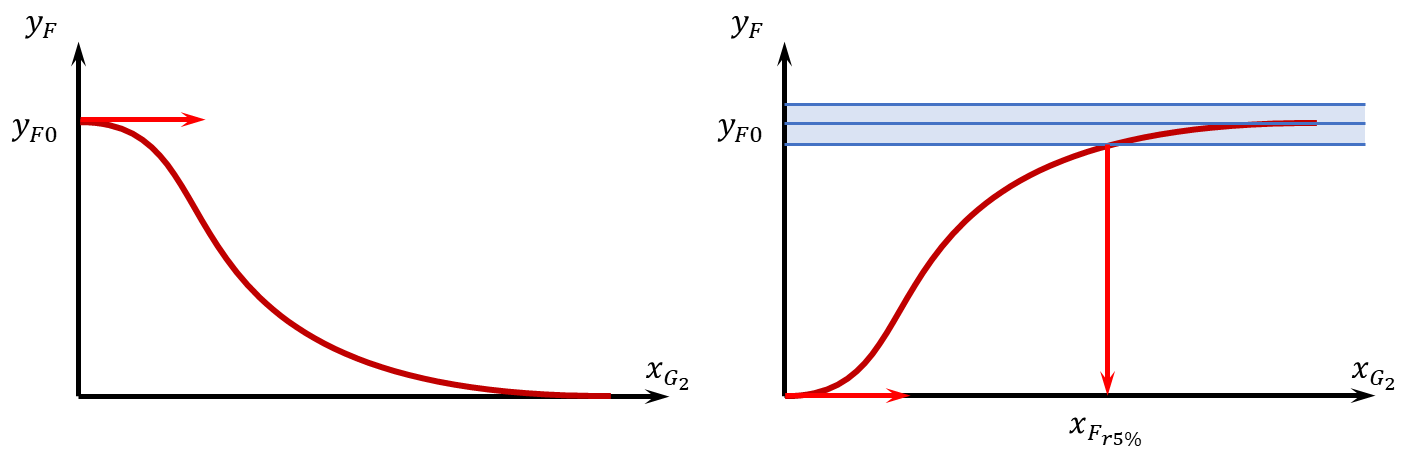
\includegraphics[width=.8\linewidth]{images/fig_05}
\end{center}
\textbf{Justifier que $K_{pF}=\dfrac{K^2_{dF}}{4}$}
En ayant fait ce choix pour $K_{pF}$, on assure un $\xi=1$ donc un système le plus rapide possible sans dépassement. 
Cela permet d'éviter les oscillations autour de la trajectoire cible et donc de limiter les problèmes de glissement. 

\end{UPSTIcorrige}


\UPSTIquestion Expliquer ce que représente $x_{F_{r5\%}}$ dans le cas de ce modèle spatial (I.8), analogue du temps de réponse à \SI{5}{\%} dans le cas d’un modèle temporel. Préciser son unité. Compte-tenu de la valeur prise précédemment pour le réglage de $K_{pF}$, donner alors une expression littérale approchée de  $x_{F_{r5\%}}$ en fonction de $K_{dF}$. Effectuer
l’application numérique et conclure sur la pertinence de la valeur numérique de $K_{dF}$, vu le contexte d’utilisation
du robot enjambeur.

\begin{UPSTIcorrige}
$x_{F_{r5\%}}$ représente la distance que met le robot à être à une distance inférieure à \SI{5}{\%} de la trajectoire. Elle s'exprime en mètres (si toutes les distance sont en mètres).

D'après l'abaque du temps de réponse à \SI{5}{\%} pour un système d'ordre 2, on a  $\omega_{0F} x_{F_{r5\%}}\simeq 5$ pour $\xi_F=1$  \textbf{(ce résultat ne me semble pas exigible dans le programme de PCSI-PSI)}. On a alors 
$x_{F_{r5\%}} \simeq \dfrac{5}{\omega_{0F} }$ $\simeq\dfrac{5}{\sqrt{K_{pF}}}$ $\simeq \dfrac{5\times 2}{K_{dF}}$ $\simeq \SI{2}{m}$.
Cela semble réaliste compte-tenu de la longueur des rangs de vignes.
\end{UPSTIcorrige}

\subsubsection{Génération des consignes d'orientation $\delta_F^*$ et $\delta_R^*$ des roues médianes}
\UPSTIobjectif{ Établir deux relations permettant de déterminer la consigne d’orientation de la roue médiane avant
$\delta_F^*$ et celle de la roue médiane arrière $\delta_R^*$ (figure A).}


\UPSTIquestion À partir des relations issues du modèle cinématique étendu du robot (figure A), de la relation issue
du modèle 1 choisi pour le comportement de $y_F\left(x_{G_2}\right)$, et en sachant que les relations (E1) et (E2) trouvées à la question 1 permettent de considérer que les valeurs des variables $y_F$ et $y_F$ sont connues si $y_{G_2}$ et $\theta$ le sont aussi (trajectoire $\mathcal{T}$ connue) :
\begin{enumerate}
\item déterminer l’expression de $y''_F$, en fonction de $\delta_F$, $\beta_F$, $\delta_R$, $\beta_R$ et $L$. Pour ce faire, commencer par exprimer $y''_F$ à partir de la relation (I.4), en tenant compte de l’hypothèse relative aux valeurs de $\delta'_F-\beta'_F$;
\item en tenant compte du point de fonctionnement souhaité, déterminer ensuite l’expression de $\delta_F$ de la roue
médiane avant 5, en utilisant la relation (I.7), puis les relations (I.4) et (E3) ;
\item en identifiant précisément les variables qui sont mesurées et estimées, et en supposant que les dispositifs
d’orientation des roues fonctionnent parfaitement et assurent ainsi que $\delta^*_F = \delta_F$, montrer alors que l’expression de $\delta^*_F$ est de la forme $\delta^*_F =C_1 \hat{\beta}_F +C_2\left(\delta_R - \hat{\beta}_R\right)+C_3 y_F + C_4 y_R$;
\item donner les expressions littérales de $C_1$, $C_2$, $C_3$ et $C_4$ en fonction de $K_{dF}$, $K_{pF}$ et $L$.
\end{enumerate}

\begin{UPSTIcorrige}
\textbf{Déterminer l’expression de $y''_F$, en fonction de $\delta_F$, $\beta_F$, $\delta_R$, $\beta_R$ et $L$}

D'après la relation (I.4), on a : $y'_F = \theta + \delta_F-\beta_F$. On  alors $y''_F =\dfrac{\dd y'_F}{\dd x_{G_2}} = \theta' + \delta_F'-\beta_F'$. Or en utilisant (I.6), on obtient 
$y''_F = \dfrac{y'_F-y'_R}{2L} + \delta_F'-\beta_F'$. En utilisant a nouveau (I.4) et (I.5), 
$y''_F = \dfrac{\left(\theta + \delta_F-\beta_F\right)-\left(\theta + \delta_R-\beta_R\right)}{2L} + \delta_F'-\beta_F'$
soit $y''_F = \dfrac{ \delta_F- \delta_R +\beta_R-\beta_F}{2L} + \delta_F'-\beta_F'$.

En tenant compte de l'hypothèse du sujet, $ \delta_F'-\beta_F'\simeq 0$ et 
$y''_F = \dfrac{ \delta_F- \delta_R +\beta_R-\beta_F}{2L}$.



\textbf{Déterminer ensuite l’expression de $\delta_F$}

D'après (I.7), on a $y''_F  + K_{dF}y'_F+K_{pF}y_F = K_{pF}y_F^*$. En utilisant (I.4),  
$y''_F  + K_{dF}\left(  \theta + \delta_F-\beta_F \right)+K_{pF}y_F = K_{pF}y_F^*$.
Enfin en utilisant (E3), 
$y''_F  + K_{dF}\left(  \dfrac{y_R-y_F}{2L} + \delta_F-\beta_F \right)+K_{pF}y_F = K_{pF}y_F^*$.

On a donc 
$K_{dF} \delta_F  = K_{pF}y_F^* - y''_F - K_{pF}y_F- K_{dF}\left(  \dfrac{y_R-y_F}{2L} -\beta_F \right)$

$\Leftrightarrow  \delta_F  = \dfrac{K_{pF}}{K_{dF}}y_F^* - \dfrac{y''_F}{K_{dF}} - \dfrac{K_{pF}}{K_{dF}}y_F- \left(  \dfrac{y_R-y_F}{2L} -\beta_F \right)$.

\textbf{Montrer que $\delta^*_F =C_1 \hat{\beta}_F +C_2\left(\delta_R - \hat{\beta}_R\right)+C_3 y_F + C_4 y_R$}

En utilisant les relations précédentes, on a 
$\delta_F  = \dfrac{K_{pF}}{K_{dF}}y_F^* - \dfrac{1}{K_{dF}}\left(  \dfrac{ \delta_F- \delta_R +\beta_R-\beta_F}{2L} \right) - \dfrac{K_{pF}}{K_{dF}}y_F- \left(  \dfrac{y_R-y_F}{2L} -\beta_F \right)$.


On peut montrer que  $\hat{\beta}_F= {\beta}_F$ et $\hat{\beta}_R= {\beta}_R$.

(En effet : $\hat{\beta}_F = \theta + \delta_F -\dfrac{\dot{y}_F}{V_{G_2}}$ 
$=\dfrac{y_R-y_F}{2L}+ \delta_F -\dfrac{\dot{y}_F}{V_{G_2}}$
$=\dfrac{y_R-y_F}{2L}+ \delta_F -\dfrac{V_{G_2}\left( \theta+\delta_F-\beta_F\right)}{V_{G_2}}$
$=\dfrac{y_R-y_F}{2L} -\left( \dfrac{y_R-y_F}{2L}-\beta_F\right)$ $=\beta_F$).


On a donc 
$\delta_F  = \dfrac{K_{pF}}{K_{dF}}y_F^* - \dfrac{1}{K_{dF}}\left(  \dfrac{ \delta_F- \delta_R +\hat{\beta}_R-\hat{\beta}_F}{2L} \right) - \dfrac{K_{pF}}{K_{dF}}y_F-   \dfrac{y_R-y_F}{2L} +\hat{\beta}_F $

$\Leftrightarrow \delta_F  = \dfrac{K_{pF}}{K_{dF}}y_F^* - \dfrac{1}{2L K_{dF}}\left(   \delta_F- \delta_R +\hat{\beta}_R-\hat{\beta}_F \right) - \dfrac{K_{pF}}{K_{dF}}y_F   -   \dfrac{y_R}{2L}+   \dfrac{y_F}{2L} +\hat{\beta}_F $

$\Leftrightarrow \delta_F  = \dfrac{K_{pF}}{K_{dF}}y_F^* 
-\dfrac{ \delta_F}{2L K_{dF}}
%+\dfrac{1}{2L K_{dF}}\left(  \hat{\beta}_F \right)  
+  \left(1+\dfrac{1}{2L K_{dF}}\right)\hat{\beta}_F
+\dfrac{1}{2L K_{dF}}\left(   \delta_R -\hat{\beta}_R \right)  
+\left( \dfrac{1}{2L}  - \dfrac{K_{pF}}{K_{dF}}\right)y_F 
- \dfrac{y_R}{2L} $

$\Leftrightarrow \delta_F  \left(1+ \dfrac{ 1}{2L K_{dF}}\right)= \dfrac{K_{pF}}{K_{dF}}y_F^* 
%+\dfrac{1}{2L K_{dF}}\left(  \hat{\beta}_F \right)  
+  \left(1+\dfrac{1}{2L K_{dF}}\right)\hat{\beta}_F
+\dfrac{1}{2L K_{dF}}\left(   \delta_R -\hat{\beta}_R \right)  
+\left( \dfrac{1}{2L}  - \dfrac{K_{pF}}{K_{dF}}\right)y_F 
- \dfrac{y_R}{2L} $

%$\Leftrightarrow \delta_F   \dfrac{ 1+2L K_{dF}}{2L K_{dF}}= 
$\Leftrightarrow \delta_F   = 
\dfrac{2L K_{pF}}{ 1+2L K_{dF}}  y_F^* 
+\hat{\beta}_F
+\dfrac{1}{ 1+2L K_{dF}} \left(   \delta_R -\hat{\beta}_R \right)  
+\dfrac{K_{dF} - 2LK_{pF}}{ 1+2L K_{dF}} y_F 
- \dfrac{ K_{dF}}{ 1+2L K_{dF}}y_R $.

On aurait donc $C_1 = 1$, $C_2 = \dfrac{1}{ 1+2L K_{dF}}$, $C_3 =\dfrac{K_{dF} - 2LK_{pF}}{ 1+2L K_{dF}} $, $C_4= - \dfrac{ K_{dF}}{ 1+2L K_{dF}} $.
\begin{flushright}
\textbf{Ne correspond pas à l'expression demandée.}
\end{flushright}
\end{UPSTIcorrige}


\end{document}
